% template - article
% here is document's settings for russian uncoment here if you do not use 'main.tex'
%% template - preamble for article
%\documentclass[a4paper,12pt]{article} % format of document, use it in 'main.tex' or here

\usepackage[T1,T2A]{fontenc}        % add eng,rus encoding support
\usepackage[utf8]{inputenc}         % add UTF8 support
\usepackage[english,russian]{babel} % add eng,rus(base) package
\usepackage{soul}                   % add l a t t r s p a c i n g
\usepackage{longtable}              % To display tables on several pages
\usepackage{booktabs}               % For prettier tables -> does not work
\usepackage{enumitem}               % advanced lists support
%\usepackage{fontspec}       % to use any font known to the operating system
%\setmainfont{PT Serif}      % set defolt font

\usepackage{amsmath, amsfonts, amssymb, amsthm, mathtools} % add math support

\usepackage{geometry}  % add document's fields correction support
\geometry{top=25mm}    % top field
\geometry{bottom=30mm} % bottom field
\geometry{left=20mm}   % left field
\geometry{right=20mm}  % right field

\linespread{1}               % length between str
\setlength{\parindent}{20pt} % red str
\setlength{\parskip}{12pt}   % length between paragraphs

\usepackage[backend=biber, style=authoryear-icomp]{biblatex} % add bibliography support
\addbibresource{$HOME/latex-templates/biblio.bib}            % path to bibliography base
\usepackage{csquotes}                                        % advanced facilities for inline and display quotations

\usepackage{indentfirst} % first paragraph with red str
\usepackage[colorinlistoftodos]{todonotes}  % allows us to write todonotes

% Must be the last command into the preamble of document.
\usepackage{hyperref} % All references in document turn into hyperlinks
\hypersetup{
unicode=true,      % Юникод в названиях разделов в PDF
colorlinks=true,   % Цветные ссылки вместо ссылок в рамках
linkcolor=blue,    % Внутренние ссылки
citecolor=green,   % Ссылки на библиографию
filecolor=magenta, % Ссылки на файлы
urlcolor=blue,     % Ссылки на URL
}

% the same for english
%% template - preamble for article
%\documentclass[a4paper,12pt]{article} % format of document, use it in 'main.tex' or here

\usepackage[T1,T2A]{fontenc}        % add eng,rus encoding support
\usepackage[utf8]{inputenc}         % add UTF8 support
\usepackage[russian,english]{babel} % add rus,eng(base) package
\usepackage{soul}                   % add l a t t r s p a c i n g
\usepackage{longtable}              % To display tables on several pages
\usepackage{booktabs}               % For prettier tables -> does not work
\usepackage{enumitem}               % advanced lists support
%\usepackage{fontspec}       % to use any font known to the operating system
%\setmainfont{PT Serif}      % set defolt font
\usepackage{graphicx}               % to embed pictures
\usepackage{subcaption}             % to show multiple figures

\usepackage{amsmath, amsfonts, amssymb, amsthm, mathtools} % add math support

\usepackage{geometry}  % add document's fields correction support
\geometry{top=25mm}    % top field
\geometry{bottom=30mm} % bottom field
\geometry{left=20mm}   % left field
\geometry{right=20mm}  % right field

\linespread{1}               % length between str
\setlength{\parindent}{20pt} % red str
\setlength{\parskip}{12pt}   % length between paragraphs

\usepackage[backend=biber, style=authoryear-icomp]{biblatex} % add bibliography support
\addbibresource{$HOME/latex-templates/biblio.bib}            % path to bibliography base
\usepackage{csquotes}                                        % advanced facilities for inline and display quotations

\usepackage{indentfirst} % first paragraph with red str
\usepackage[colorinlistoftodos]{todonotes}   % allows us to write todonotes

% Must be the last command into the preamble of document.
\usepackage{hyperref} % All references in document turn into hyperlinks
\hypersetup{
unicode=true,      % Юникод в названиях разделов в PDF
colorlinks=true,   % Цветные ссылки вместо ссылок в рамках
linkcolor=blue,    % Внутренние ссылки
citecolor=green,   % Ссылки на библиографию
filecolor=magenta, % Ссылки на файлы
urlcolor=blue,     % Ссылки на URL
}


\subsection{Sample of text formating}
This is test text.

\subsection{Samples of formating}
\textbf{some bold text}
\textit{some italic text}
\emph{some emphatic text}
\underline{some underline text}

\so{SOME SO TEXT}

\subsection{Sample of quotation}
``some text with quotation marks'' and  <<some text with quotation marks>>

\subsection{Sample of pictures}
This is a picture:
\begin{figure}[!hbtp]
    \begin{center}
    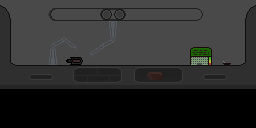
\includegraphics[width=0.8\textwidth]{pics/astro-ship-engener.png}
    \end{center}
    \caption{This is a test picture.\label{Picture_example}}
\end{figure}

\subsection{Samples of lists\label{List_examples}}

\subsubsection{Sample of ordered list}
\begin{enumerate}
    \item item1
        \begin{enumerate}
            \item item1.1
        \end{enumerate}
    \item item2
    \item item3
\end{enumerate}

\subsubsection{Sample of unordered list}
\begin{itemize}
    \item item1
        \begin{itemize}
            \item item1.1
        \end{itemize}
    \item item2
    \item item3
\end{itemize}

\subsection{Samples of lables}
In section \ref{List_examples} I am talking about Lists. About picture, see \ref{Picture_example}.

\subsection{Samples of bibliography management}
As \parencite{example-book} says, use bibliograpy in \LaTeX{}! And this is a reference to ``Article'' : \parencite{example-article}. Alsow see this book \parencite{example-incollection}.

Using \texttt{biblatex} you can display a bibliography divided into sections, depending on citation type.  Let's cite! Einstein's journal paper \parencite{example-article} and Dirac's book \parencite{example-book} are physics-related items.

Next, \textit{The \LaTeX\ Companion} book \parencite{example-book}, Donald Knuth's website \parencite{example-online}, \textit{The Bite Of Python} \parencite{chitlur2014} are \LaTeX-related items; but the others, Donald Knuth's items, \cite{example-inbook} are dedicated to programming.

\subsection{Samples of formulas}
This is a formula: $2 + 2 = 4$.

This is an other formula:
\[2 + 2 = 4\]

These are formulas:
\[\int_{-\infty}^{+\infty} e^{-\frac{x^2}{2}} = \sqrt{2 \pi}\]

\[x_n, x^k, x_n^k, x^k_n, x_{i + j}^{2022}\]

\[(x^i)^n\]

\[x^{i^n}\]
